\documentclass{article}
\usepackage[utf8]{inputenc}
\usepackage[letterpaper,margin=1in]{geometry}
\usepackage{graphicx}
\usepackage{listings}
\usepackage{color}
\usepackage{hyperref}
\usepackage{multirow}

\definecolor{mine}{rgb}{0,0,0.7}
\hypersetup{
    colorlinks=true,
    linkcolor=mine,
    citecolor=mine,
    urlcolor=mine,
    pdftitle={SPOTs Imager},
}

\definecolor{dkgreen}{rgb}{0,0.6,0}
\definecolor{gray}{rgb}{0.5,0.5,0.5}
\definecolor{mauve}{rgb}{0.58,0,0.82}

\lstset{frame=tb,
  language=matlab,
  aboveskip=3mm,
  belowskip=3mm,
  showstringspaces=false,
  columns=flexible,
  basicstyle={\small\ttfamily},
  numbers=none,
  numberstyle=\tiny\color{gray},
  keywordstyle=\color{blue},
  commentstyle=\color{dkgreen},
  stringstyle=\color{mauve},
  breaklines=true,
  breakatwhitespace=true,
  tabsize=3
}

\title{Scanning Imager Guide}
\author{Mark Menesses}
\date{15 September 2020}

\begin{document}

\maketitle

\tableofcontents
\newpage

\section{Overview}
The SPOTs scanning imager allows for programmatic imaging of SPOTs across a large area (30cm x 30cm).
\section{Hardware}
The system is comprised of a motorized X-Y stage and an imaging head.
The system is controlled using Gcode fed into a GRBL controller.
\subsection{Stage}
The current stage in use is the \href{https://openbuilds.com/builds/openbuilds-acro-system.5416/}{ACRO 55} purchased from \href{https://openbuilds.com/}{OpenBuilds}.
This stage offers X and Y movement over a 12''x12'' area.
Some specs:

\begin{tabular}{l l}
     Drive System: & Belt Driven GT2 timing belts \\
     Machine Accuracy: & 0.003"~0.007" (0.10mm~0.20mm) (This seems off. Might be more like $\pm$0.05mm) \\
     Footprint: & 20" x 20" (500mm x 500mm) \\
     Motors: & NEMA 17 \\
     Controller: & OpenBuilds BlackBox \\
\end{tabular}


\begin{figure}[!h]
    \centering
    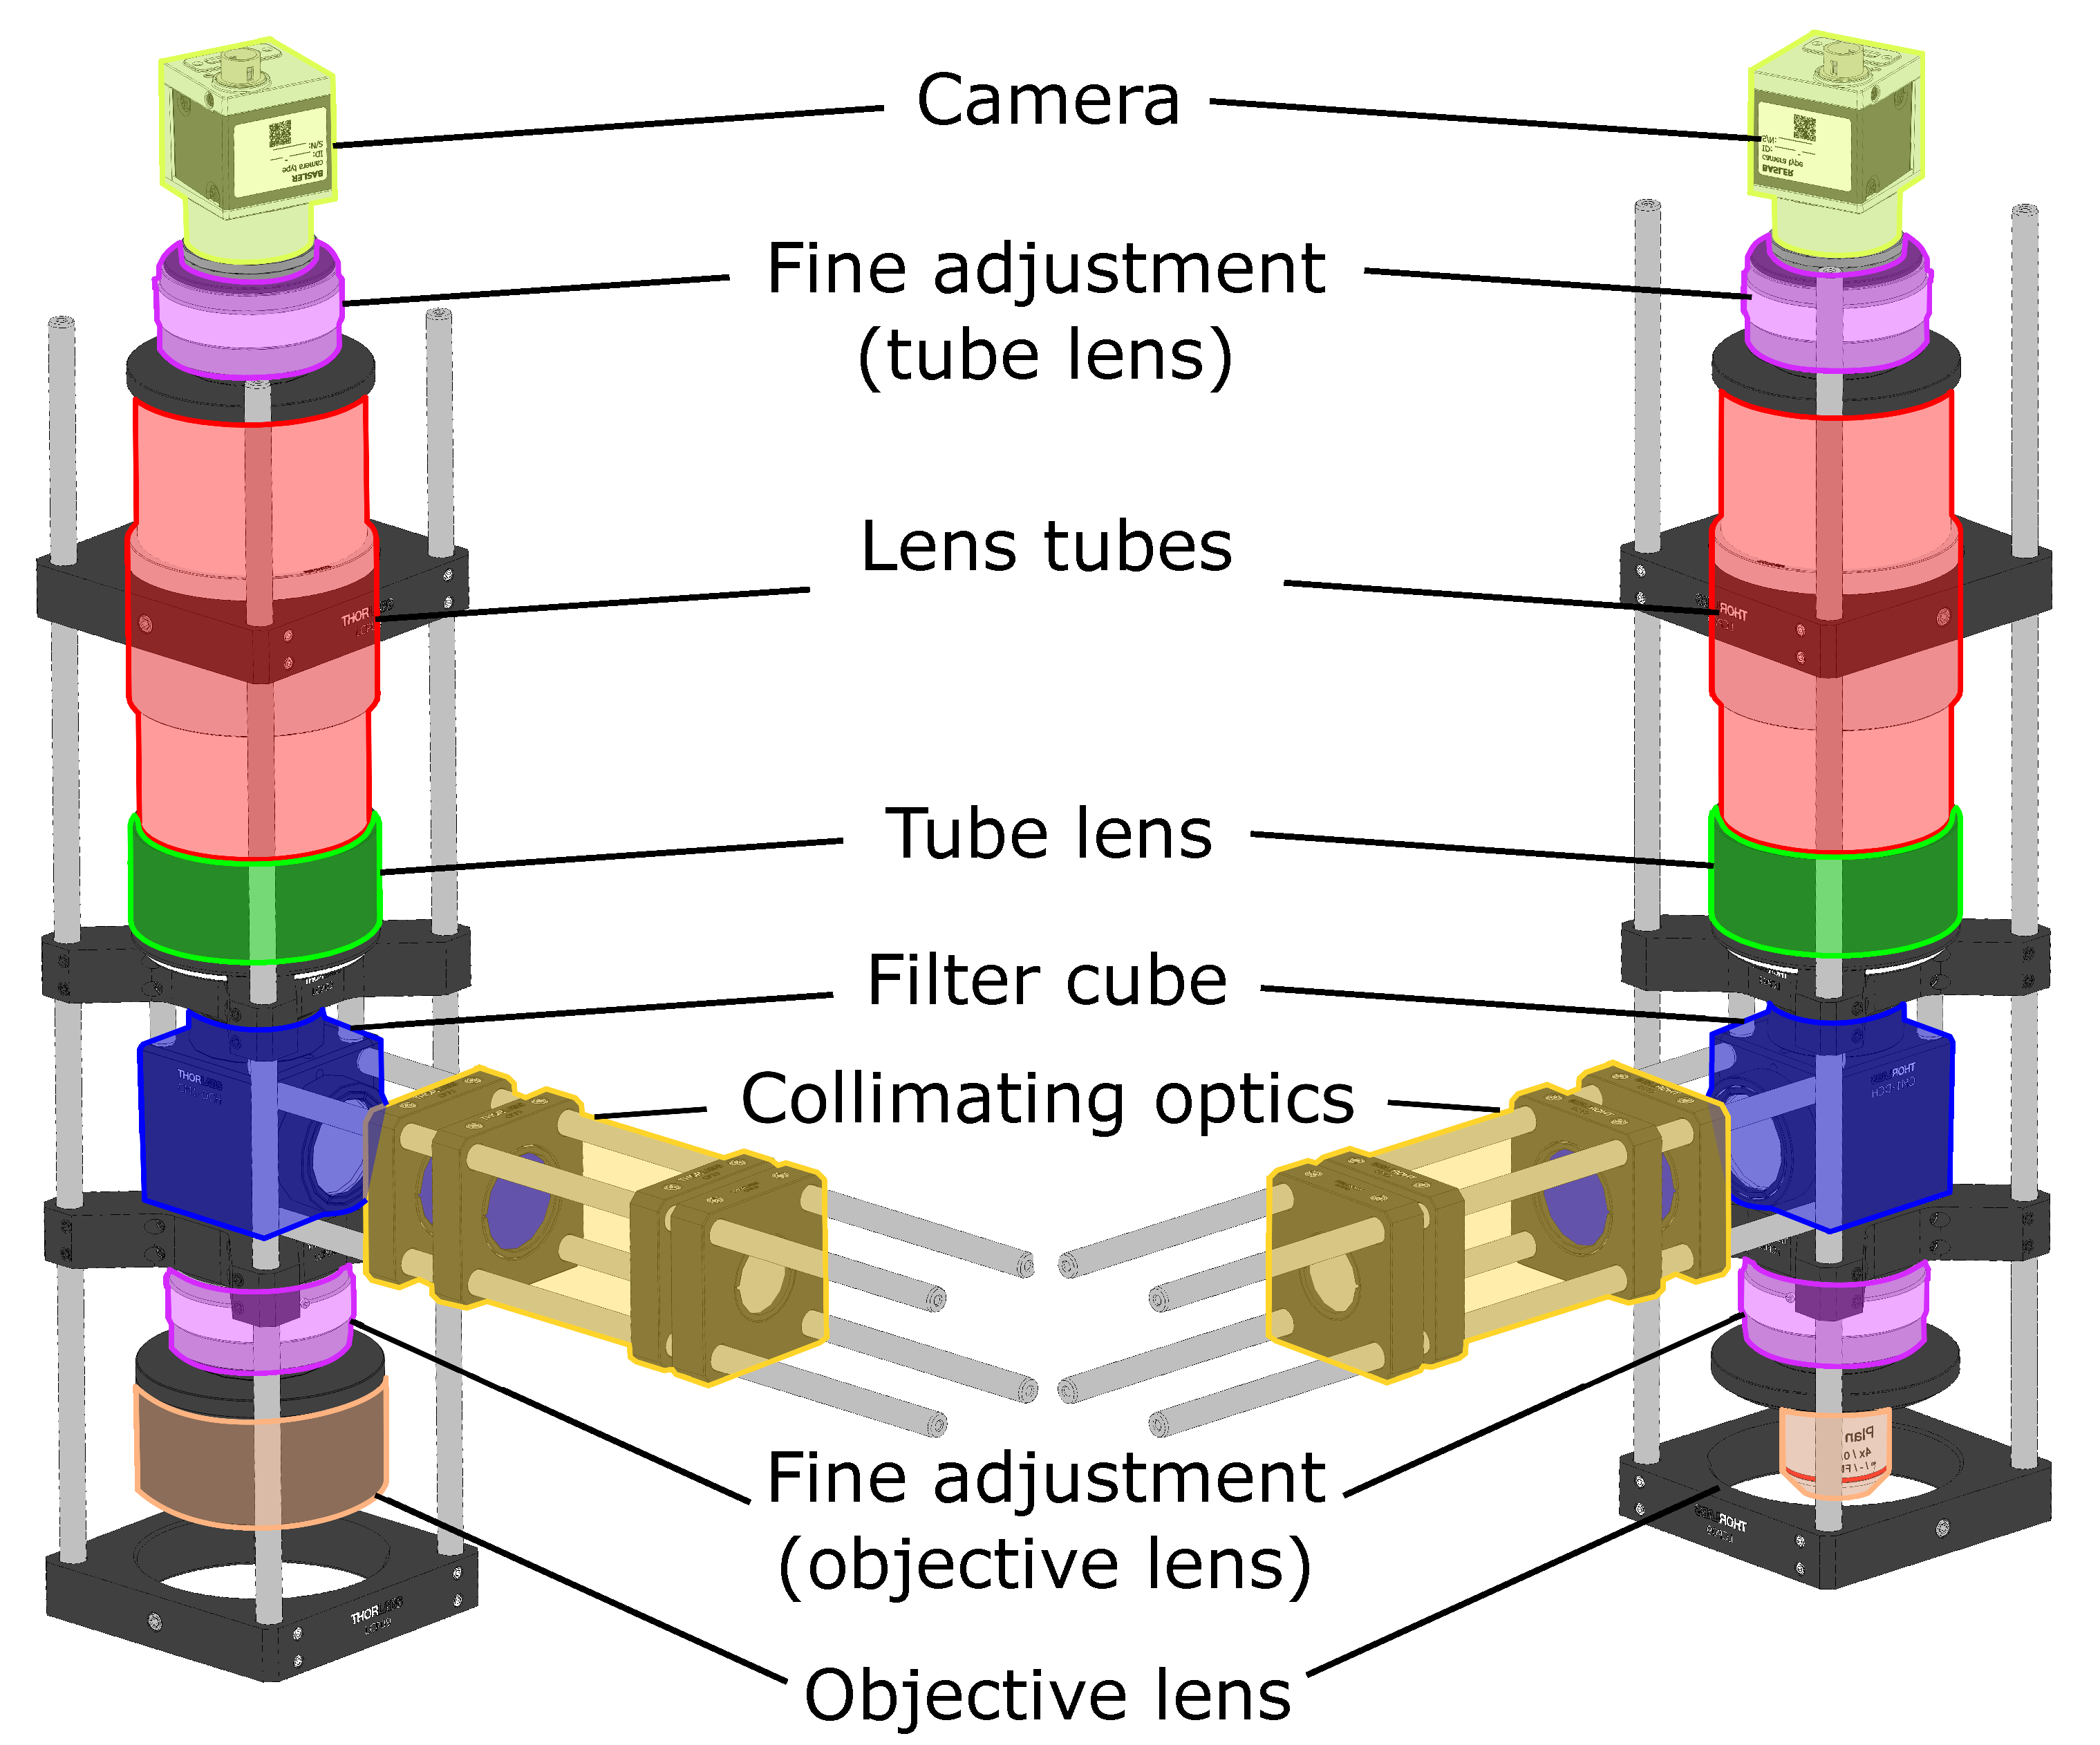
\includegraphics[width=0.75\columnwidth]{imager_sketch.eps}
    \caption{Sketch of imaging components. The left configuration shows an achromatic lens used as the objective, while the right shows an infinity corrected microscope objective in use.}
    \label{fig:sketch}
\end{figure}

\subsection{Camera}
	
A variety of cameras may be used with a preference for smaller, C-mount cameras for weight purposes.
The camera should be supported by MATLAB's Image Acquisition toolbox for ease of integration.
Currently, we use a \href{https://www.baslerweb.com/en/products/cameras/area-scan-cameras/ace/aca3800-14uc/}{Basler acA3800-14uc} (specs below).

\begin{tabular}{l l}
    Sensor Size: & 6.4mm x 4.6 mm \\
    Resolution: & 3840 px x 2748 px (10 MP) \\
    Pixel Size: & 1.67 $\mu$m x 1.67 $\mu$m \\
    Max. Frame Rate (at full res.): & 14 fps \\
    Pixel Bit Depth: & 12 bits
\end{tabular}

\subsection{Optics}
A custom set of optics is being used to achieve a range of magnifications and enable the use of epifluorescence.
Optical components for the collimation of the excitation light were duplicated from the Thorlabs WFA2001 module.
Two lenses are used in the system, an objective lens and a tube lens, between which sets up an infinity space between them in which we introduce our epi-illumination.
The available lenses are listed in Table \ref{tab:lenses}.
The range of magnifications available for a given lens pair is listed in Table \ref{tab:magnifications}.

\begin{table}[!h]
\centering
\begin{tabular}{c c c c c c}
    \textbf{Lens}  & \textbf{Description} & \textbf{Thorlabs PN} & \textbf{Focal Length} & \textbf{Working Distance} & \textbf{Magnification} \\
    A & Achromatic lens & AC508-100-A & 100 mm & 89.0 mm & --- \\
	B & Achromatic lens & AC508-150-A & 150 mm & 140.4 mm & --- \\
	C & Achromatic lens & AC508-180-A & 180 mm & 172.7 mm & --- \\
	D & Achromatic lens & AC508-200-A & 200 mm & 193.7 mm & --- \\
	E & Plan N 4x & RMS4X & 180 mm & 18.5 mm & 4x 
\end{tabular}
\caption{Lens choices and properties}
\label{tab:lenses}
\end{table}

\bgroup
\def\arraystretch{1.35}
\begin{table}[!h]
    \centering
    \begin{tabular}{c c|c|c|c|c}
           & & \multicolumn{4}{c}{\textbf{Tube Lens}} \\
           & &  A   &  B   &  C   &  D  \\
           \hline
        \multirow{5}{*}{\rotatebox[origin=c]{90}{\textbf{Objective Lens}}} & A & ---  & 1.50 & 1.80 & 2.00 \\ \cline{2-6}
         & B & 0.67 & --- & 1.20 & 1.33 \\ \cline{2-6}
         & C & 0.56 & 0.83 & --- & 1.11 \\ \cline{2-6}
         & D & 0.50 & 0.75 & 0.90 & --- \\ \cline{2-6}
         & E & 2.22 & 3.33 & 4.00 & 4.444 \\
    \end{tabular}
    \caption{Magnifications achieved by varying lens combinations}
    \label{tab:magnifications}
\end{table}
\egroup

\section{Setup}
\subsection{Select magnification}
Use Table \ref{tab:magnifications} to select the appropriate lenses for the desired magnification.
\subsection{Install lenses}
Lenses installed on the system as shown in Figure \ref{fig:sketch}.
Each achromatic lens is mounted within its own threaded housing.
To install these lenses in the objective position, they should be screwed into the thread adapter below the fine focus adjustment at the bottom of the assembly (the exterior threads will be facing upwards).

\subsection{Focus optics}
\subsection{}
Prior to operation, the user should select the lenses (Table \ref{tab:lenses}) which will give the appropriate magnification, as given in Table \ref{tab:magnifications}.
The camera must be placed at the working distance of the tube lens.
Currently, a series of threaded lens tubes provides coarse adjustment of this distance, while fine adjustment

\section{Image acquisition workflow}

\section{In progress}
\subsection{Epifluorescence}
We have optics setup that should allow for epifluorescence, but this remains to be tested.
One item to be considered still is the light source.
We can either choose a specific wavelength for a given application, or use a broadband source and filter.
The modular nature of our system requires a rather lightweight source, such as a small LED. One issue may be heating of the light source.
We could consider using the controller PWM pin to turn our light on and off between images.
\subsection{Image stitching}
We have not yet chosen a software for image stitching.
As this is a post-processing step, many options are available.




\section{Cost}
\begin{table}[!h]
\centering
\begin{tabular}{cccccc}
\textbf{Vendor} & \textbf{Part Number} & \textbf{Brief Description}              & \textbf{Qty} & \textbf{Unit Price} & \textbf{Subtotal} \\
 & & & & \textbf{(USD)} & \textbf{(USD)} \\
Thorlabs        & AC508-100-A          & Achromatic Lens, f=100mm                & 1            & 113                       & 113                     \\
Thorlabs        & AC508-150-A          & Achromatic Lens, f=150mm                & 1            & 113                       & 113                     \\
Thorlabs        & AC508-180-A          & Achromatic Lens, f=150mm                & 1            & 113                       & 113                     \\
Thorlabs        & AC508-200-A          & Achromatic Lens, f=100mm                & 1            & 113                       & 113                     \\
Thorlabs        & AL2018-A             & Collimating optics                      & 1            & 240                       & 240                     \\
Thorlabs        & CM1-DCH              & Filter cube                             & 1            & 175                       & 175                     \\
Thorlabs        & CP33                 & Lens housing                            & 3            & 17                        & 51                      \\
Thorlabs        & CPN20                & Lens housing                            & 1            & 34                        & 34                      \\
Thorlabs        & ER1                  & Cage rails                              & 4            & 5                         & 20                      \\
Thorlabs        & ER05                 & Cage rails                              & 4            & 5                         & 20                      \\
Thorlabs        & ER8                  & Cage rails                              & 4            & 12                        & 48                      \\
Thorlabs        & ER12                 & Cage rails                              & 4            & 17                        & 68                      \\
Thorlabs        & LBF254-040-A         & Collimating optics                      & 2            & 57                        & 114                     \\
Thorlabs        & LBF254-100-A         & Collimating optics                      & 1            & 57                        & 57                      \\
Thorlabs        & LCP02                & Cage plate                              & 2            & 42                        & 84                      \\
Thorlabs        & LCP09                & Cage plate                              & 2            & 46                        & 92                      \\
Thorlabs        & MD480                & Dichroic                                & 1            & 237                       & 237                     \\
Thorlabs        & MF434-17             & Excitation Filter                       & 1            & 258                       & 258                     \\
Thorlabs        & MF630-69             & Emission Filter                         & 1            & 258                       & 258                     \\
Thorlabs        & RMS4X                & 4x microscope objective                 & 1            & 146                       & 146                     \\
Thorlabs        & SM1A2                & Thread adapter                          & 3            & 27                        & 81                      \\
Thorlabs        & SM1A9                & Thread adapter                          & 1            & 20                        & 20                      \\
Thorlabs        & SM1L03               & Filter mount/lens tube                  & 4            & 13                        & 52                      \\
Thorlabs        & SM1ZM                & Fine adjustment for optics              & 2            & 176                       & 352                     \\
Thorlabs        & SM2A32               & Thread adapter                          & 1            & 28                        & 28                      \\
Thorlabs        & SM2L10               & Lens housing                            & 4            & 31                        & 124                     \\
Thorlabs        & LCP01B               & Mounting hardware                       & 2            & 32                        & 64                      \\
Thorlabs        & SM2T20               & Lens tube                               & 2            & 41                        & 82                      \\
Thorlabs        & SM2T10               & Lens tube                               & 1            & 39                        & 39                      \\
Thorlabs        & SM2T2                & Lens tube                               & 1            & 38                        & 38                      \\
Thorlabs        & SM2M10               & Lens tube                               & 1            & 30                        & 30                      \\
Thorlabs        & SM2M15               & Lens tube                               & 1            & 31                        & 31                      \\
Thorlabs        & SM2M20               & Lens tube                               & 1            & 33                        & 33                      \\
Edmund Optics   & 89-992               & C-Mount USB Camera                      & 1            & 695                       & 695                     \\
OpenBuilds      & 2365-Bundle          & Stage frame components & 1            & 290                       & 290                     \\
OpenBuilds      & 2790-Kit             & Stage controller                        & 1            & 190                       & 190                     \\
OpenBuilds      & 623                  & Stage motors                            & 3            & 18                        & 54                      \\
OpenBuilds      & 591-Set              & 24V power supply                        & 1            & 70                        & 70                      \\
                &                      &                                         &              &                           & \textbf{4627}          
\end{tabular}
\caption{Bill of materials}
\end{table}

\begin{figure}[!h]
    \centering
    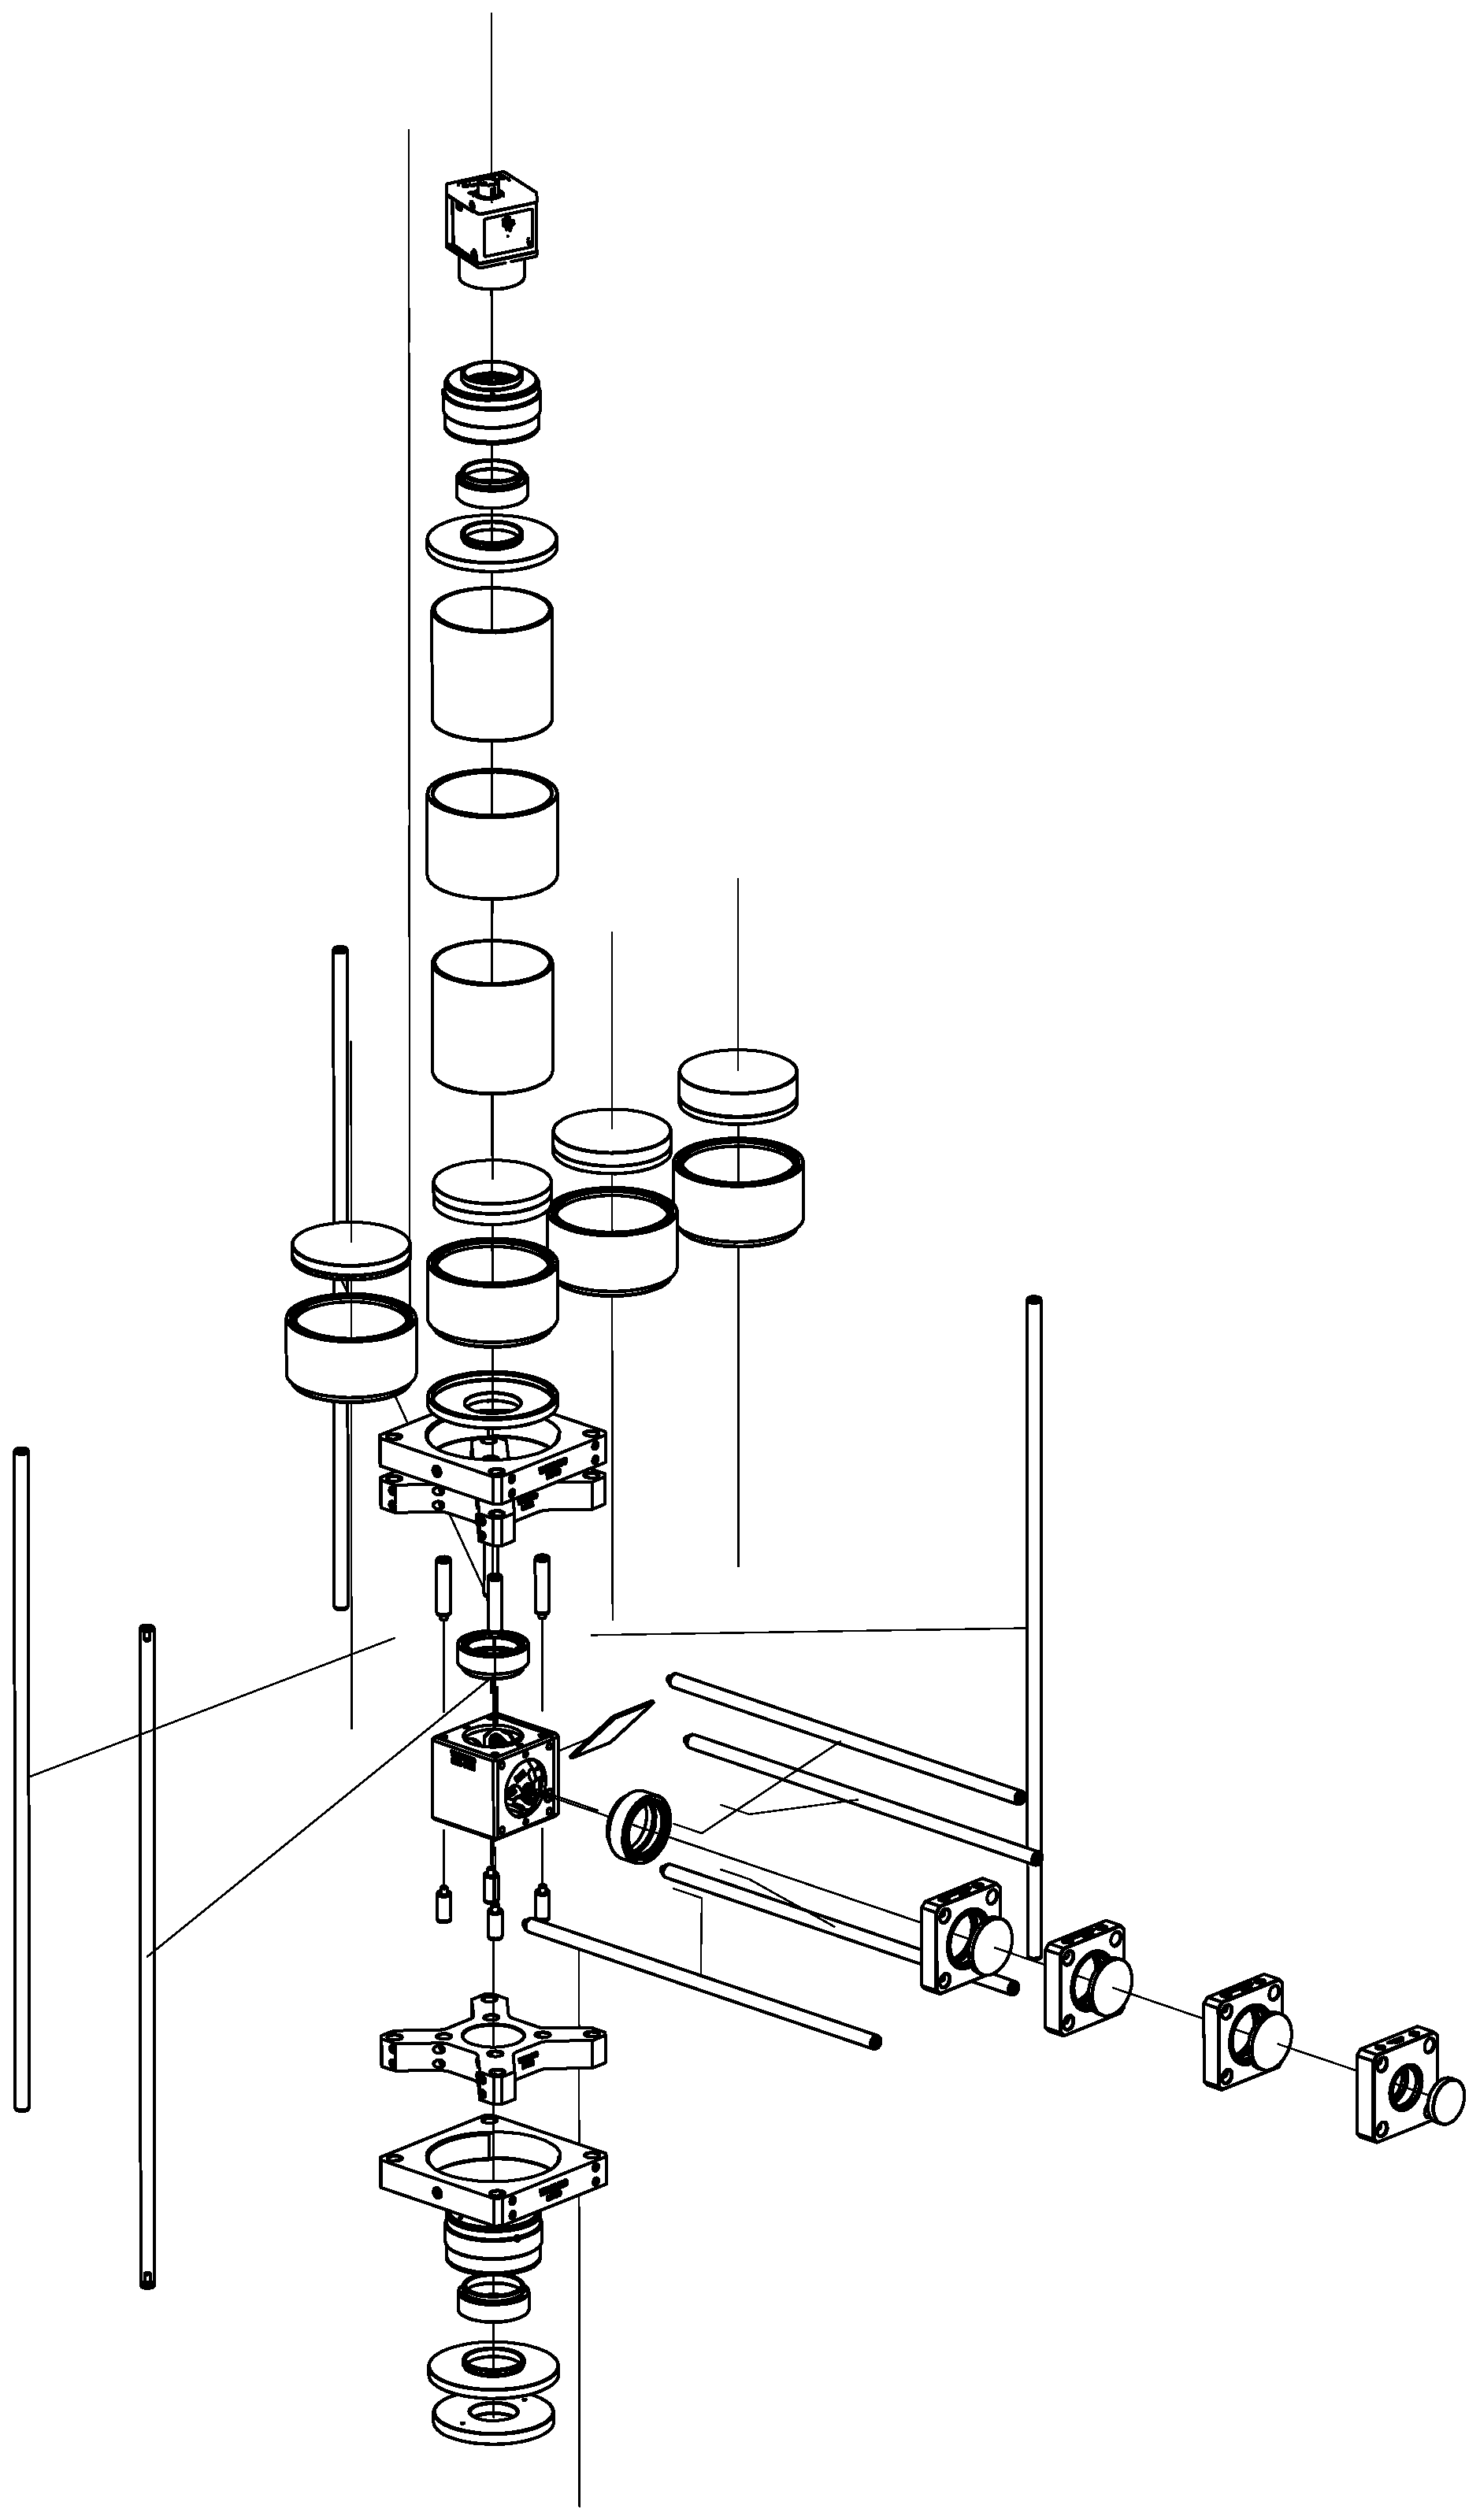
\includegraphics[width = 0.5\columnwidth]{optics_assembly_illustrated_exploded.eps}
    \caption{Exploded schematic of optical assembly}
    \label{fig:my_label}
\end{figure}


\section{MATLAB Code:}
    \subsection{Main Script}
        \begin{lstlisting}
% SCANNINGIMAGER.M
% AUTHOR: MARK MENESSES
% DATE: 1 SEPTEMBER 2020
% Tested with R2019b
%
% Requirements:
% - Image Acquisition Toolbox
% - GenICam Support Package
%        (https://www.mathworks.com/hardware-support/gentl.html)
% 
% For use with BlackBox Controller (or maybe any controller running GRBL?)
% and Basler acA3800-14uc camera.
% 
% Info on GRBL: https://github.com/gnea/grbl/wiki/Grbl-v1.1-Configuration
%

%% Start fresh
clc
clear all
close all

%% Prompt user input
[idealx,idealy] = inputPointsOfInterest;

idealPoints = inputRegPoints;

feedrate = 1000;

%% CAMERA OPTIONS
% Connect to device (valid formats: 'BayerBG8', 'BayerBG12', 'Mono8')
vid = videoinput('gentl',1,'BayerBG8');

% Common properties to tweak. See all available properties using the
% command "get(getselectedsource(vid))"
set(vid.Source,...
    'BalanceWhiteAuto', 'Off',...
    'DecimationHorizontal', 1,...
    'DecimationVertical', 1,...
    'ExposureAuto', 'Once',...
    'Gain', 0,...
    'GainAuto', 'Off',...
    'ShutterMode', 'Rolling');
%     'ExposureTime', 35000,...

% Only capture one image at a time
set(vid,'FramesPerTrigger',1);


%% Connect to controller

% Define serial port and establish settings
ser = serial('COM5');
set(ser,'BaudRate',115200);
set(ser,'Parity','none');
set(ser,'DataBits',8);
set(ser,'StopBit',1);

% Open port and initialize
fopen(ser);
fprintf(ser,'\r\n\r\n');
pause(2)
getResponse(ser); % "error:9" is expected due to use of soft limits

% Need to home to unlock
fprintf(ser,'$H\n');
ismoving = true;
while ismoving
    ismoving = ~isStopped(ser);
    disp('Homing...')
    pause(0.1)
end
disp('Homed!')

% Set zero at homed position
fprintf(ser,'G10P1L20X0Y0Z0\n');
getResponse(ser);

%% Jog for registration points

% Using GUI applet to jog and capture registration points
% Passing in video and serial port
realPoints = jogapplet(vid,ser);

% Return to absolute programming
fprintf(ser,'G90\n');

% Reset some camera values
set(vid.Source,'DecimationHorizontal',1)
set(vid.Source,'DecimationVertical',1)

% Generate spot map and transform using registration points
tform_matrix = fitgeotrans(idealPoints,realPoints,'affine');
[machinex,machiney] = transformPointsForward(tform_matrix,idealx,idealy);


%% Beginning loop
check4Alarm(ser)

% Looping through all coordinates
for i=1:numel(idealx)
    xloc = machinex(i);
    yloc = machiney(i);
    
    % Move to position
    movestage(ser,xloc,yloc,feedrate)
    waituntilstopped(ser)
    check4Alarm(ser)
    
    % Check current position
    checkposition = false;
    n=0;
    while checkposition == false
        [~,~,here] = getWCoMPos(ser);
        if and(round(abs(here(1)-xloc),3)<0.045,round(abs(here(2)-yloc),3)<0.045)
            % First check if we think we're within 45um of our point
            checkposition = true;
        elseif n==1
            % If not within tolerance at first try, just reissue the gcode
            % command.
            movestage(ser,xloc,yloc,feedrate)
            waituntilstopped(ser)
        elseif n > 5
            % Raise error after 5 attempts if unsuccessful
            error("Can't get to position")
        else
            % If off after reissuing original command, try moving away a
            % litte, then reissue command
            movestage(ser,xloc+1+rand*3,yloc+1+rand*3,100)
            waituntilstopped(ser)
            movestage(ser,xloc,yloc,feedrate)
            waituntilstopped(ser)
        end
    end
    
    % Throw out any existing images
    if vid.FramesAvailable>0
        data = getdata(vid);
        data = [];
    end
    
    % Take image
    imgname = [num2str(idealx(i),'%02d'),'_',num2str(idealy(i),'%02d'),...
        '-img',num2str(i,'%04d'),'.png'];
    start(vid)
    % Wait up to 30 seconds for successful capture
    startwatch = now;
    stopwatch = 0;
    while and(vid.FramesAvailable==0,stopwatch<30)
        pause(0.1)
        stopwatch = (now - startwatch)*24*60*60;
    end
    
    % Save image (with CreationTime metadata) if successful.
    if vid.FramesAvailable > 0
        [img,~,frameinfo] = getdata(vid,1);
        imwrite(img,imgname,'CreationTime',datestr(frameinfo.AbsTime));
    elseif vid.FramesAvailable == 0
        disp('Frame not captured!')
    end
    
end

% Write CSV file with image number and coordinates
A=zeros(numel(idealx),3);
for i = 1:numel(idealx)
    A(i,1)=i;
    A(i,2)=machinex(i);
    A(i,3)=machiney(i);
end
T = array2table(A,'VariableNames',{'ImageNo.','X_pos','Y_pos'});
tablename = [strrep(strrep(datestr(datetime),' ','_'),':',''),...
    '_img_positions.csv'];
writetable(T,tablename,'Delimiter',',');

fclose(ser);
delete(vid);
delete(ser);
clear vid ser

\end{lstlisting}
    \subsection{Functions}
        \subsubsection{getWCoMPos}
\begin{lstlisting}
function [WCo,MPos,position] = getWCoMPos(serial_port)
% Returns Working Coordinate (WCo), Machine Position (MPos), and position.
% WCo is returned by controller only every ~1s or so. We thus loop here
% until we have received it. WCo is NOT the actual coordinates to be input
% into GCode commands.
    got_it = false;
    while ~got_it
        fprintf(serial_port,'?\n');
        pause(0.1)
        response = getResponse(serial_port);
		% Parse through response looking for WCO and MPos.
        if contains(response,"WCO")
            response = strsplit(response,'<');
            response = response(end);
            response = strsplit(response(contains(response,'>')),'>');
            out = strsplit(response(1),'|');
            coord = strsplit(out(contains(out,"WCO")),':');
            WCo = str2double(strsplit(coord(2),','));
            pos = strsplit(out(contains(out,"MPos")),':');
            MPos = str2double(strsplit(pos(2),','));
            position = MPos - WCo;
            got_it = true;
        else
            WCo = NaN;
            MPos = NaN;
            position = NaN;
        end
    end
    if isequal(MPos, [0 0 0])
        error('MACHINE NOT HOMED! POSITION UNRELIABLE!')
    end
end

\end{lstlisting}
\subsubsection{isStopped}
\begin{lstlisting}
function stopped = isStopped(serial_port)
% Check position two times and see if we're still moving.
    posA = getMPos(serial_port);
    pause(0.25)
    posB = getMPos(serial_port);
    stopped = isequal(posA,posB);
end

\end{lstlisting}
\subsubsection{waituntilstopped}
\begin{lstlisting}
function waituntilstopped(serial_port)
    while ~isStopped(serial_port)
    end
end

\end{lstlisting}
\subsubsection{jogapplet}
\begin{lstlisting}
function reg_points = jogapplet(VideoInput,SerialPort)
% Launches jog applet.
% Displays a user interface figure populated with the following panels and
% components:
%   - Video Panel (vidpnl): holds video start and stop buttons
%   - Registration Panel (regpnl): holds point registration buttons and
%         displays for registered points. Also holds submit points button.
%   - Jog Panel (jogpnl): holds directional jog buttons and movement
%         increment selection.
%   - Alarm Panel (alarmpnl): holds alarm indicator and button to reset/unlock
%         the controller following an alarm.

    % Open figure
    fig = uifigure('Name','Registration Preview','Position',[100 100 1260 700]);
    
	% Create axes that will house the video preview
	ax = uiaxes(fig,'Position',[10 10 960 687],...
        'Visible','off');
    
	% Setup global temp_points variable to be updated with registration buttons.
    global temp_points
    temp_points = zeros(3,2)*NaN;
    
	% Change video source parameters to fit video
    set(VideoInput.Source,'DecimationHorizontal',4)
    set(VideoInput.Source,'DecimationVertical',4)
	% Empty image object to be filled by video later
    im = image(ax,zeros([687, 960],'uint8'));
    
	% Create panel for video buttons
    vidpnl = uipanel(fig,'Position',[1000 600 200 100]);
	% Direct video preview to previous image object on button click.
    vidstart = uibutton(vidpnl,...
        'ButtonPushedFcn',@(vidstart,event) preview(VideoInput,im),...
        'Position',[10 10 85 80],...
        'FontSize',16,...
        'Text',{'Start','Video'},...
        'HorizontalAlignment','center');
	% Close existing video preview on button click.
    vidstop = uibutton(vidpnl,...
        'ButtonPushedFcn',@(vidstop,event) closepreview(VideoInput),...
        'Position',[105 10 85 80],...
        'FontSize',16,...
        'Text',{'Stop','Video'},...
        'HorizontalAlignment','center');
    
	% Create panel for registration buttons.
    regpnl = uipanel(fig,'Position',[1000 335 200 260]);
	% Run registerPoint function on button click for point 1.
    regbtn1 = uibutton(regpnl,...
        'ButtonPushedFcn',@(regbtn1,event) registerPoint(SerialPort,1),...
        'Position',[10 195 60 60],...
        'FontSize',14,...
        'Text',{'Reg 1'},...
        'HorizontalAlignment','center');
	% Run registerPoint function on button click for point 2.
    regbtn2 = uibutton(regpnl,...
        'ButtonPushedFcn',@(regbtn2,event) registerPoint(SerialPort,2),...
        'Position',[10 130 60 60],...
        'FontSize',14,...
        'Text',{'Reg 2'},...
        'HorizontalAlignment','center');
	% Run registerPoint function on button click for point 3.
    regbtn3 = uibutton(regpnl,...
        'ButtonPushedFcn',@(regbtn3,event) registerPoint(SerialPort,3),...
        'Position',[10 65 60 60],...
        'FontSize',14,...
        'Text',{'Reg 3'},...
        'HorizontalAlignment','center');
	% Create a sub-panels to hold the registered coordinates.
	% These are continually updated in a loop below.
    coord1pnl = uipanel(regpnl,'Position',[80 195 110 60]);
    x1lab = uilabel(coord1pnl,'Position',[5 30 30 30],...
        'Text','X1:','FontSize',14,'FontWeight','bold');
    x1coord = uilabel(coord1pnl,'Position',[45 30 60 30],...
        'Text','---','FontSize',14,'FontWeight','bold');
    y1lab = uilabel(coord1pnl,'Position',[5 0 30 30],...
        'Text','Y1:','FontSize',14,'FontWeight','bold');
    y1coord = uilabel(coord1pnl,'Position',[45 0 60 30],...
        'Text','---','FontSize',14,'FontWeight','bold');
    coord2pnl = uipanel(regpnl,'Position',[80 130 110 60]);
    x2lab = uilabel(coord2pnl,'Position',[5 30 30 30],...
        'Text','X2:','FontSize',14,'FontWeight','bold');
    x2coord = uilabel(coord2pnl,'Position',[45 30 60 30],...
        'Text','---','FontSize',14,'FontWeight','bold');
    y2lab = uilabel(coord2pnl,'Position',[5 0 30 30],...
        'Text','Y2:','FontSize',14,'FontWeight','bold');
    y2coord = uilabel(coord2pnl,'Position',[45 0 60 30],...
        'Text','---','FontSize',14,'FontWeight','bold');
    coord3pnl = uipanel(regpnl,'Position',[80 65 110 60]);
    x3lab = uilabel(coord3pnl,'Position',[5 30 30 30],...
        'Text','X3:','FontSize',14,'FontWeight','bold');
    x3coord = uilabel(coord3pnl,'Position',[45 30 60 30],...
        'Text','---','FontSize',14,'FontWeight','bold');
    y3lab = uilabel(coord3pnl,'Position',[5 0 30 30],...
        'Text','Y3:','FontSize',14,'FontWeight','bold');
    y3coord = uilabel(coord3pnl,'Position',[45 0 60 30],...
        'Text','---','FontSize',14,'FontWeight','bold');
	% Submits registered points and closes applet.
    submitbtn = uibutton(regpnl,...
        'ButtonPushedFcn',@(submitbtn,event) submitpoints,...
        'Position',[10 5 180 55],...
        'FontSize',14,...
        'Text',{'Submit','points'},...
        'HorizontalAlignment','center');
    
	% Create panel for jog controlls.
    jogpnl = uipanel(fig,'Position',[1000  90 200 240]);
	% Make list of increments at which stage can move. Starts unselected.
    inc_list = uilistbox(jogpnl,...
        'Items', {'0.1','1.0','10','100'},...
        'Position',[130 5 60 90],...
        'FontSize',16,...
        'Value',{});
    inc_label = uilabel(jogpnl,...
        'HorizontalAlignment','right',...
        'Position',  [10 25 110 60],...
        'FontSize', 16,...
        'Text',{'Jog Increment','(mm)'});
	% Make button for movement in x+ direction
    xP = uibutton(jogpnl,'push',...
        'ButtonPushedFcn',@(xP,event) xpbtn(SerialPort,inc_list.Value),...
        'Text', 'X+',...
        'FontSize',18,...
        'FontWeight','bold',...
        'Position',[135 140 60 60]);
	% Make button for movement in x- direction
    xM = uibutton(jogpnl,'push',...
        'ButtonPushedFcn',@(xN,event) xmbtn(SerialPort,inc_list.Value),...
        'Text', 'X-',...
        'FontSize',18,...
        'FontWeight','bold',...
        'Position',[5 140 60 60]);
	% Make button for movement in y+ direction
    yP = uibutton(jogpnl,'push',...
        'ButtonPushedFcn',@(yP,event) ypbtn(SerialPort,inc_list.Value),...
        'Text', 'Y+',...
        'FontSize',18,...
        'FontWeight','bold',...
        'Position',[70 175 60 60]);
	% Make button for movement in y- direction
    yM = uibutton(jogpnl,'push',...
        'ButtonPushedFcn',@(yM,event) ymbtn(SerialPort,inc_list.Value),...
        'Text', 'Y-',...
        'FontSize',18,...
        'FontWeight','bold',...
        'Position',[70 105 60 60]);
    
	% Create panel for alarm status and reset.
    alarmpnl = uipanel(fig,'Position',[1000 20 200 65]);
    alarmlabel = uilabel(alarmpnl,...
        'Text','Alarm:',...
        'HorizontalAlignment','right',...
        'VerticalAlignment','center',...
        'FontSize',16,...
        'FontWeight','Bold',...
        'Position',[10 15 60 35]);
    alarmlight = uilamp(alarmpnl,...
        'Color',[1 1 1],...
        'Position',[alarmlabel.Position(1)+alarmlabel.Position(3)+5,...
        alarmlabel.Position(2), alarmlabel.Position(4),...
        alarmlabel.Position(4)]);
    alarmresetbtn = uibutton(alarmpnl,...
        'ButtonPushedFcn',@(alarmresetbtn,event) unlockcontroller(SerialPort),...
        'Text','Re-home',...
        'Position',[alarmlight.Position(1)+alarmlight.Position(3)+15,...
        alarmlight.Position(2),...
        alarmpnl.Position(3)-alarmlight.Position(3)-alarmlight.Position(1)-25,...
        alarmlight.Position(4)]);
    
	% Force all elements defined above to be drawn
    drawnow
    
	% Loop to continually update whether points have been submitted, check
	% alarm status, and update any registered points.
    global pointsgood
    pointsgood = false;
    while ~pointsgood
        if check4Alarm(SerialPort)
            alarmlight.Color = [1 0 0];
        else
            alarmlight.Color = [1 1 1];
        end
        if ~isnan(temp_points(1,1))
            x1coord.Text = num2str(temp_points(1,1));
            y1coord.Text = num2str(temp_points(1,2));
        end
        if ~isnan(temp_points(2,1))
            x2coord.Text = num2str(temp_points(2,1));
            y2coord.Text = num2str(temp_points(2,2));
        end
        if ~isnan(temp_points(3,1))
            x3coord.Text = num2str(temp_points(3,1));
            y3coord.Text = num2str(temp_points(3,2));
        end
        reg_points = temp_points;
        pause(0.1)
    end
    
    if pointsgood
        closepreview;
        closereq;
    end
end

\end{lstlisting}
\subsubsection{xpbtn}
\begin{lstlisting}
function xpbtn(serial_port,increment)
% For use in jog applet
% Button response function for x+ movement. Sends command to move stage
% at given increment.
    command = ['G91X',num2str(increment),'Y0F2000'];
    fprintf(serial_port,command);
    pause(0.1)
    getResponse(serial_port)
end

\end{lstlisting}
\subsubsection{xmbtn}
\begin{lstlisting}
function xmbtn(serial_port,increment)
% For use in jog applet
% Button response function for x- movement. Sends command to move stage
% at given increment.
    command = ['G91X-',num2str(increment),'Y0F2000'];
    fprintf(serial_port,command);
    pause(0.1)
    getResponse(serial_port)
end

\end{lstlisting}
\subsubsection{ypbtn}
\begin{lstlisting}
function ypbtn(serial_port,increment)
% For use in jog applet
% Button response function for y+ movement. Sends command to move stage
% at given increment.
    command = ['G91X0Y',num2str(increment),'F2000'];
    fprintf(serial_port,command);
    pause(0.1)
    getResponse(serial_port)
end

\end{lstlisting}
\subsubsection{ymbtn}
\begin{lstlisting}
function ymbtn(serial_port,increment)
% For use in jog applet
% Button response function for y- movement. Sends command to move stage
% at given increment.
    command = ['G91X0Y-',num2str(increment),'F2000'];
    fprintf(serial_port,command);
    pause(0.1)
    getResponse(serial_port)
end

\end{lstlisting}
\subsubsection{registerPoint}
\begin{lstlisting}
function registerPoint(serial_port,number)
% For use in jog applet
% Gets Machine Coordinates and modifies global temp_points variable
    global temp_points
    [~,~,position] = getWCoMPos(serial_port);
    temp_points(number,1:2) = position(1:2);
end
\end{lstlisting}
\subsubsection{submitpoints}
\begin{lstlisting}
function submitpoints
% For use in jog applet
% Signals that all registration points are satisfactory as determined by the
% user, then closes applet and video preview
    global pointsgood
    pointsgood = true;
    pause(0.5)
%     closepreview;
%     closereq;
end
\end{lstlisting}
\subsubsection{movestage}
\begin{lstlisting}
function movestage(serial_port,x_coord,y_coord,feedrate)
% Use this function to send movement commands. Prevents movements that are
% out of ranget as to avoid alarms and resetting mid-run.
    [wco, mpos, position] = getWCoMPos(serial_port);
    movement = [x_coord y_coord 0] - position;
%     disp(['Movement:', num2str(movement)])
%     disp(['-mpos:',num2str(-mpos)])
%     disp(['movement+mpos:',num2str(movement+mpos)])
%     disp(['wco:',num2str(wco)])
    if sum(movement > -mpos)~=0
        % Prevents movement too far in the positive directions. This is
        % related to the soft-limits in GRBL settings.
        error('Movement out of range!')
    elseif sum(movement+mpos < wco-2) ~= 0
        % Prevents movements too far in the negative directions, which
        % would eventually hit the limit switches. Allows for movements
        % -2mm past the homed position. GRBL settings dictate the standoff
        % from the limit switches. We typically run these at 5mm.
        error('Movement out of range!')
    else
        fprintf(serial_port,['G1X',num2str(x_coord,'%0.4f'),'Y',...
            num2str(y_coord,'%0.4f'),'F',num2str(feedrate)])
    end
end


\end{lstlisting}
\subsubsection{getResponse}
\begin{lstlisting}
function response = getResponse(serial_port)
% Get any response available from the controller.
    response = "";
    if serial_port.BytesAvailable > 0
        while serial_port.BytesAvailable > 0
            response = response + fscanf(serial_port);
        end
        disp(response)
    end
end

\end{lstlisting}
\subsubsection{check4Alarm}
\begin{lstlisting}
function alarm = check4Alarm(serial_port)
% Look for alarm status
    fprintf(serial_port,'?\n');
    pause(0.01)
    response = getResponse(serial_port);
    if contains(response,"Alarm")
        alarm = true;
        error("Alarm triggered!")
    else
        alarm = false;
    end
end

\end{lstlisting}
\subsubsection{unlockcontroller}
\begin{lstlisting}
function unlockcontroller(serial_port)
    fprintf(serial_port,'$H\n')
    pause(0.1)
    if check4Alarm(serial_port)
        error('Unlock failed!')
    end
end

\end{lstlisting}


\begin{table}[!h]
    \centering
        \begin{tabular}{c c c}
            \textbf{Tube Lens} & \textbf{Objective Lens} & \textbf{Magnification} \\
            A & D & 0.50 \\
            A & C & 0.56 \\
            A & B & 0.67 \\
            B & D & 0.75 \\
            B & C & 0.83 \\
            C & D & 0.90 \\
            D & C & 1.11 \\
            C & B & 1.20 \\
            D & B & 1.33 \\
            B & A & 1.50 \\
            C & A & 1.80 \\
            D & A & 2.00 \\
            A & E & 2.22 \\
            B & E & 3.33 \\
            C & E & 4.00 \\
            D & E & 4.44
        \end{tabular}
    \caption{Magnifications achieved by varying lens combinations}
    \label{tab:magnifications2}
\end{table}

\end{document}
